\documentclass[11pt]{article}
\usepackage[T1]{fontenc}
\usepackage[margin=1in]{geometry}
\usepackage{graphicx}
\usepackage{amssymb}
\usepackage{bbold}
\usepackage{amsmath}
\usepackage{booktabs}
\usepackage{listings}
\usepackage[hidelinks]{hyperref}

\newcommand{\ind}{\mathbb{1}}
\newcommand{\Normal}{\mathcal{N}}
\newcommand{\BF}{\mathrm{BF}}
\DeclareMathOperator*{\argmax}{arg\,max}
\DeclareMathOperator{\RSS}{RSS}
\lstset{language=R,basicstyle=\ttfamily\small,columns=fullflexible,
        keepspaces=true,showstringspaces=false,breaklines=true,
        frame=single}

\title{The slider model}
\author{William Denault}
\date{September 2026}

\begin{document}
\maketitle

\section{Introduction}

Consider a single-nucleotide polymorphism (SNP) with genotype
$x\in\{0,1,2\}$, coded as the number of copies of a specified allele,
and a quantitative phenotype $y$. Write
\begin{align}
\Delta_{01} &= E(y\mid x=1)-E(y\mid x=0),\\
\Delta_{12} &= E(y\mid x=2)-E(y\mid x=1).
\end{align}
An additive genotype--phenotype relationship satisfies
$\Delta_{01}=\Delta_{12}$. For an allele that increases the phenotype,
partial recessivity corresponds to $0<\Delta_{01}<\Delta_{12}$,
whereas partial dominance corresponds to
$\Delta_{01}>\Delta_{12}>0$. Complete recessivity and complete dominance
allow one of these two increments to be zero.

We use a \emph{slider} parameter to represent these relationships by
changing the numerical position of the heterozygous genotype. The
phenotype values and genotype-group memberships remain unchanged.
This document describes the one-SNP model, its implemented estimation
procedure, its extension to single-effect regression and variational
empirical Bayes, the sampling distribution of the estimated slider
under additivity, and an optional Bayesian comparison of additive
and nonadditive effects.

\section{Model}

For independent observations $(x_i,y_i)$, $i=1,\ldots,n$, define the slider model as
\begin{align}
y_i &= \alpha+\beta f_\delta(x_i)+\epsilon_i,
    \label{eq:model}\\
f_\delta(x) &= x+\delta\ind_{\{x=1\}}
 =\begin{cases}
 0,&x=0,\\
 1+\delta,&x=1,\\
 2,&x=2,
 \end{cases}
    \label{eq:coding}\\
\epsilon_i &\overset{\mathrm{iid}}{\sim}\Normal(0,\sigma^2),\\
\beta &\sim\Normal(0,\sigma_0^2),\qquad -1\leq\delta\leq1.
    \label{eq:prior}
\end{align}
The residual variance $\sigma^2$ and prior variance $\sigma_0^2$ are
positive and held fixed in the one-SNP calculations below. In the
multi-SNP extension they may instead be estimated within iterative
Bayesian stepwise selection (IBSS), as described in
Section~\ref{sec:slider-veb}. The Gaussian prior on $\beta$ is the
single-effect prior used in SuSiE~\cite{wang2020susie}.

Let $\mu_k=E(y\mid x=k,\alpha,\beta,\delta)$. Then
\begin{equation}
(\mu_0,\mu_1,\mu_2)
 =\bigl(\alpha,\alpha+\beta(1+\delta),\alpha+2\beta\bigr),
\end{equation}
so that
\begin{equation}
\Delta_{01}=\beta(1+\delta),\qquad
\Delta_{12}=\beta(1-\delta),\qquad
\mu_2-\mu_0=2\beta.
\end{equation}
Consequently, $\delta=-1$ gives recessive coding $(0,0,2)$,
$\delta=0$ gives additive coding $(0,1,2)$, and $\delta=1$ gives
dominant coding $(0,2,2)$, relative to the counted allele. Negative
$\beta$ reverses the direction of the phenotypic effect.

The bound on $\delta$ ensures that the heterozygote mean lies between
the two homozygote means. Thus, the model covers monotone increasing
or decreasing genotype means, including equality at an endpoint. It
does not cover overdominance or underdominance, where the heterozygote
mean lies outside this interval. Algebraically, the model can also be
written as
\begin{equation}
E(y\mid x)=\alpha+a x+d\ind_{\{x=1\}},
\qquad a=\beta,\quad d=\beta\delta,\quad |d|\leq|a|.
\end{equation}
This is a constrained parameterization of additive and dominance
effects. The parameter $\delta$ describes the position of the
\emph{heterozygote}; it does not change the homozygote codes.

\section{Posterior distribution of the effect at a fixed slider}
\paragraph{Centering and treatment of the intercept}

Set $h_i=\ind_{\{x_i=1\}}$, and let $\bar y$, $\bar x$, and $\bar h$
denote the corresponding sample means. With an intercept, define
\begin{equation}
y_i^c=y_i-\bar y,\qquad
x_i^c=x_i-\bar x,\qquad
h_i^c=h_i-\bar h,
\end{equation}
and, for any fixed $\delta$,
\begin{equation}
z_i(\delta)=x_i^c+\delta h_i^c
 =f_\delta(x_i)-(\bar x+\delta\bar h).
\label{eq:centered-design}
\end{equation}
Centering is equivalent to integrating the intercept under a common
flat prior $p(\alpha)\propto1$ for the model comparisons below. The
arbitrary intercept-prior constant cancels in these comparisons.
The calculations use the likelihood on the centered subspace;
centering does not imply that the centered errors are independent.

Write $\mathbf y^c=(y_1^c,\ldots,y_n^c)^\top$ and
$\mathbf z_\delta=(z_1(\delta),\ldots,z_n(\delta))^\top$. Apart from a
factor independent of $\beta$ and $\delta$, the intercept-integrated
likelihood is
\begin{equation}
L(\beta,\delta)\propto
\exp\left\{-\frac{1}{2\sigma^2}
\|\mathbf y^c-\beta\mathbf z_\delta\|^2\right\}.
\label{eq:likelihood}
\end{equation}
When the intercept is fixed to zero, the same formulas apply with
$y_i^c=y_i$, $x_i^c=x_i$, and $h_i^c=h_i$, and the reported intercept
is zero. Both the phenotype and transformed predictor are treated
consistently in either case.

For fixed $\delta$, define
\begin{equation}
S_\delta=\mathbf z_\delta^\top\mathbf z_\delta,
\qquad
T_\delta=\mathbf z_\delta^\top\mathbf y^c.
\end{equation}
Combining equations~\eqref{eq:prior} and~\eqref{eq:likelihood} and
completing the square gives
\begin{align}
V_\delta
 &=\left(\frac{1}{\sigma_0^2}+
              \frac{S_\delta}{\sigma^2}\right)^{-1},
    \label{eq:posterior-variance}\\
m_\delta
 &=V_\delta\frac{T_\delta}{\sigma^2}
  =\frac{T_\delta}{S_\delta+\sigma^2/\sigma_0^2},
    \label{eq:posterior-mean}\\
\beta\mid\mathbf y,\mathbf x,\delta
 &\sim\Normal(m_\delta,V_\delta).
    \label{eq:posterior}
\end{align}
Dependence on the fixed variances is suppressed in the conditioning
notation. This is an exact Gaussian posterior at the specified
$\delta$, with the intercept integrated out when present.

The posterior mean of the intercept at this same $\delta$ is
\begin{equation}
\widehat\alpha_\delta
 =\bar y-m_\delta(\bar x+\delta\bar h).
\label{eq:intercept}
\end{equation}
The posterior mean fitted values are therefore
\begin{equation}
\widehat y_i(\delta)
 =\widehat\alpha_\delta+m_\delta f_\delta(x_i).
\label{eq:fitted}
\end{equation}

\section{Learning the slider by marginal likelihood}

The main fitting routine places no prior on $\delta$. In our
implementation, integrating over a slider prior increased the
computation time by a factor of 10--20. Instead, we estimate $\delta$
by maximum marginal likelihood in an empirical-Bayes fashion:
we first integrate out $\beta$ under its Gaussian prior and then
find a slider value that maximizes the resulting marginal likelihood.

Let $M_\varnothing$ denote the no-SNP model $\beta=0$, with the same
treatment of the intercept. For a fixed slider, define
\begin{equation}
\BF(\delta)
 =\frac{p(\mathbf y\mid\mathbf x,\delta)}
        {p(\mathbf y\mid M_\varnothing)},
\end{equation}
where the numerator integrates $\beta$, and both models integrate
the intercept if it is included. Following the original SuSiE manuscript gives
\begin{align}
\ell(\delta):=\log\BF(\delta)
 &=-\frac12\log\left(1+\frac{\sigma_0^2S_\delta}{\sigma^2}\right)
   +\frac{\sigma_0^2T_\delta^2}
    {2\sigma^2(\sigma^2+\sigma_0^2S_\delta)}
    \label{eq:logbf}\\
 &=\frac12\left\{\log\left(\frac{V_\delta}{\sigma_0^2}\right)
                   +\frac{m_\delta^2}{V_\delta}\right\}.
\end{align}
The denominator does not depend on $\delta$, so the estimate is
\begin{equation}
\widehat\delta
 \in\argmax_{-1\leq\delta\leq1}\ell(\delta).
\label{eq:delta-estimate}
\end{equation}
The reported effect estimate is $\widehat\beta=m_{\widehat\delta}$,
with conditional posterior standard deviation
$\sqrt{V_{\widehat\delta}}$. This standard deviation does not
include uncertainty in the estimated slider.

The main computational advantage is that only a one-dimensional
optimization is required. The implementation finds its stationary
points algebraically. Define
\begin{equation}
u_i=\frac{\sigma_0}{\sigma}x_i^c,\qquad
v_i=\frac{\sigma_0}{\sigma}h_i^c,\qquad
w_i=\frac{y_i^c}{\sigma},
\end{equation}
and the five quantities
\begin{equation}
A=1+\mathbf u^\top\mathbf u,\quad
B=\mathbf u^\top\mathbf v,\quad
D=\mathbf v^\top\mathbf v,\quad
C=\mathbf u^\top\mathbf w,\quad
E=\mathbf v^\top\mathbf w.
\end{equation}
With
\begin{equation}
Q(\delta)=A+2B\delta+D\delta^2
          =1+\|\mathbf u+\delta\mathbf v\|^2,
\qquad U(\delta)=C+E\delta,
\end{equation}
equation~\eqref{eq:logbf} becomes
\begin{equation}
\ell(\delta)=\frac12\left\{\frac{U(\delta)^2}{Q(\delta)}
                                      -\log Q(\delta)\right\}.
\end{equation}
Since $Q(\delta)$ is 1 plus a sum of squares, $Q(\delta)\geq1$.
The derivative can be written as
\begin{equation}
\ell'(\delta)=\frac{P(\delta)}{Q(\delta)^2},\qquad
P(\delta)=EU(\delta)Q(\delta)
 -\{U(\delta)^2+Q(\delta)\}(B+D\delta).
\end{equation}
Expanding gives a cubic polynomial
\begin{align}
P(\delta)&=p_0+p_1\delta+p_2\delta^2+p_3\delta^3,\\
p_0&=ACE-B(C^2+A),\\
p_1&=AE^2-D(C^2+A)-2B^2,\\
p_2&=BE^2-CDE-3BD,\\
p_3&=-D^2.
\label{eq:cubic}
\end{align}
The routine evaluates $\ell$ at all real roots in $(-1,1)$ and
at both endpoints. The candidate with the largest value is selected.
Thus the maximization does not assume that the marginal likelihood is
unimodal, and includes boundary solutions corresponding to complete
dominance or recessivity.

In the base-R implementation, the polynomial coefficients are first
divided by their maximum absolute value, and the roots are computed
using \texttt{polyroot()}. A computed root $r$ is treated as real when
$|\operatorname{Im}(r)|<10^{-7}\{1+|\operatorname{Re}(r)|\}$.
Only five inner products are required, costing $O(n)$ work, after
which each objective evaluation and the cubic calculation have cost
independent of the sample size. A cubic has at most three distinct
real roots; including the endpoints $-1,1$ and the extra candidate
$0$ gives at most six candidate values. Thus the overall one-SNP
calculation scales linearly with sample size. If the derivative
polynomial is identically zero, the objective is constant and any
allowed slider, including zero, is a maximizer.

\section{From slider SER to variational empirical Bayes}
\label{sec:slider-veb}

The one-SNP calculation extends to a single-effect regression (SER)
with uncertainty over which SNP has an effect. Fitting this SER model
by empirical Bayes (EB) to the expected residuals of the other effects
then gives a block coordinate-ascent algorithm for a variational
empirical-Bayes (VEB) objective. The argument follows the general
additive-effects construction of Wang et al.~\cite{wang2018susie},
Appendix B, especially Proposition 2. Here ``additive effects'' means
that the component contributions are summed; each component may have
a nonadditive genotype coding.

The distinction between SNP-specific and shared sliders is essential.
Within one SER component we fit one slider for each candidate SNP.
In the sum of $L$ components these parameters are
$\Delta=(\delta_{\ell j})$, with a separate slider for every
component--SNP pair. They are model parameters estimated by EB.
The latent variables are the selected SNP identities and their effect
sizes.

\subsection{Working coordinates and a slider SER model}

We condition on the observed genotype matrix. To retain the
intercept-integrated convention used above, let
$\mathbf U\in\mathbb R^{n\times N}$ have orthonormal columns spanning
the orthogonal complement of $\mathbf 1$, where $N=n-1$. Thus
$\mathbf U^\top\mathbf U=I_N$ and
$\mathbf U\mathbf U^\top=I_n-\mathbf 1\mathbf 1^\top/n$.
Define
\begin{equation}
\widetilde{\mathbf y}=\mathbf U^\top\mathbf y,\qquad
\mathbf z_j(\delta)
 =\frac{\mathbf U^\top(\mathbf x_j+\delta\mathbf h_j)}{s_j},
\qquad h_{ij}=\ind_{\{x_{ij}=1\}}.
\label{eq:veb-working-design}
\end{equation}
No explicit construction of $\mathbf U$ is needed: inner products in
these coordinates equal the corresponding centered inner products.
Without an intercept take $\mathbf U=I_n$ and $N=n$.
The scales $s_j>0$ are fixed functions of the genotypes, independent
of $\delta$. Taking $s_j=1$ gives the raw-scale model above; taking
$s_j$ to be the additive genotype standard deviation matches the
scaling convention in \texttt{susieSlide}. Constant predictors are
excluded when this latter convention is used. The Gaussian effect
prior is defined on the chosen scale.

For a response $\mathbf r\in\mathbb R^N$, the slider SER model is
\begin{align}
J&\sim\operatorname{Categorical}(\pi_1,\ldots,\pi_p),
 &\beta&\sim\Normal(0,V),\qquad J\perp\beta,\nonumber\\
\mathbf r\mid J=j,\beta,\boldsymbol\delta
 &\sim\Normal\{\beta\mathbf z_j(\delta_j),\sigma^2 I_N\},
 &\delta_j&\in\mathcal D_j.
\label{eq:veb-ser-model}
\end{align}
Here $V>0$, $\sigma^2>0$, and the prior weights are fixed, with
$\pi_j>0$ and $\sum_j\pi_j=1$. Ordinarily
$\mathcal D_j=[-1,1]$; a genotype-count rule can instead impose
$\mathcal D_j=\{0\}$. These constraints depend only on the observed
genotypes. There is exactly one selected SNP in this component,
although a slider is specified for every candidate SNP.

For any fixed $\boldsymbol\delta$, put
\begin{align}
S_j(\delta)&=\|\mathbf z_j(\delta)\|^2,
 &T_j(\delta)&=\mathbf z_j(\delta)^\top\mathbf r,\nonumber\\
v_j(\delta)&=\left\{V^{-1}+S_j(\delta)/\sigma^2\right\}^{-1},
 &m_j(\delta)&=v_j(\delta)T_j(\delta)/\sigma^2.
\label{eq:veb-ser-moments}
\end{align}
Integration over $\beta$ gives
\begin{equation}
\BF_j(\delta;V,\sigma^2)
 =\left\{1+\frac{VS_j(\delta)}{\sigma^2}\right\}^{-1/2}
 \exp\left\{\frac{VT_j(\delta)^2}
 {2\sigma^2\{\sigma^2+VS_j(\delta)\}}\right\}.
\label{eq:veb-ser-bf}
\end{equation}
Thus, with $p_0(\mathbf r;\sigma^2)$ the $\Normal(0,\sigma^2 I_N)$
density, the SER marginal likelihood and exact conditional posterior
are
\begin{align}
M(\mathbf r;\boldsymbol\delta,V,\sigma^2)
 &=p_0(\mathbf r;\sigma^2)
   \sum_{j=1}^p\pi_j\BF_j(\delta_j;V,\sigma^2),
\label{eq:veb-ser-evidence}\\
a_j:=\Pr(J=j\mid\mathbf r,\boldsymbol\delta)
 &=\frac{\pi_j\BF_j(\delta_j;V,\sigma^2)}
 {\sum_{k=1}^p\pi_k\BF_k(\delta_k;V,\sigma^2)},
\label{eq:veb-ser-weights}\\
\beta\mid J=j,\mathbf r,\boldsymbol\delta
 &\sim\Normal\{m_j(\delta_j),v_j(\delta_j)\}.
\label{eq:veb-ser-posterior}
\end{align}
The variances are suppressed in the posterior conditioning notation.

\subsection{Why independent slider maximizations solve the SER EB problem}

\paragraph{Proposition 1 (SNP-specific slider EB update).}
For fixed $V$, $\sigma^2$, and $\boldsymbol\pi$, choose
\begin{equation}
\widehat\delta_j\in\argmax_{\delta\in\mathcal D_j}
       \BF_j(\delta;V,\sigma^2),\qquad j=1,\ldots,p.
\label{eq:veb-separate-maxima}
\end{equation}
Then $\widehat{\boldsymbol\delta}$ maximizes the SER marginal
likelihood in equation~\eqref{eq:veb-ser-evidence} over
$\mathcal D_1\times\cdots\times\mathcal D_p$.

\paragraph{Proof.}
Each summand in equation~\eqref{eq:veb-ser-evidence} depends on only
one slider. For every admissible $\boldsymbol\delta$,
\begin{equation}
\sum_j\pi_j\BF_j(\delta_j;V,\sigma^2)
 \leq\sum_j\pi_j\BF_j(\widehat\delta_j;V,\sigma^2).
\label{eq:veb-separability-proof}
\end{equation}
The null density is positive and independent of
$\boldsymbol\delta$, so the same inequality holds for $M$.
Continuity on the compact allowed intervals ensures that maximizers
exist. This proves the result.\hfill$\square$

The cubic maximization already derived in equation~\eqref{eq:cubic}
therefore solves each required one-dimensional problem. No posterior
SNP weight is needed in that maximization: the evidence is a sum of
independently adjustable nonnegative terms. The posterior weights
are recomputed from equation~\eqref{eq:veb-ser-weights} afterwards.
If a \emph{single} slider were shared across candidate SNPs, the
correct objective would instead be
$\sum_j\pi_j\BF_j(\delta;V,\sigma^2)$; separate candidate-wise
maximizations would not solve that different model.

\subsection{The sum-of-single-effects model and its ELBO}

Let the $L$ pairs $(J_\ell,\beta_\ell)$ be independent a priori,
with $J_\ell\sim\operatorname{Categorical}(\boldsymbol\pi)$ and
$\beta_\ell\sim\Normal(0,V_\ell)$. Define
\begin{equation}
\boldsymbol\eta_\ell
 =\beta_\ell\mathbf z_{J_\ell}(\delta_{\ell J_\ell}),\qquad
\widetilde{\mathbf y}=\sum_{\ell=1}^L\boldsymbol\eta_\ell
      +\boldsymbol\epsilon,\qquad
\boldsymbol\epsilon\sim\Normal(0,\sigma^2 I_N).
\label{eq:veb-sum-model}
\end{equation}
For every fixed $\Delta$, this specifies a proper probability model
on the working coordinates. Equivalently, the prior on
$\boldsymbol\eta_\ell$ is a mixture over $p$ Gaussian single-effect
directions, with directions determined by the sliders. This is a
special case of the general additive-effects model in Appendix B.2
of Wang et al.~\cite{wang2018susie}.

We use the variational family
\begin{equation}
q(J_1,\beta_1,\ldots,J_L,\beta_L)
  =\prod_{\ell=1}^Lq_\ell(J_\ell,\beta_\ell).
\label{eq:veb-family}
\end{equation}
Each factor is unrestricted on the pair $(J_\ell,\beta_\ell)$;
it does not factorize over candidate SNPs. Write $p_\ell$ for the
categorical--Gaussian prior on this pair and
$\theta=(\Delta,V_1,\ldots,V_L,\sigma^2)$. The objective is
\begin{align}
\mathcal F(q,\theta)
 &=E_q\log p(\widetilde{\mathbf y}\mid J,\beta,\Delta,\sigma^2)
   -\sum_{\ell=1}^L\operatorname{KL}(q_\ell\|p_\ell)
\label{eq:veb-elbo}\\
 &=\log p(\widetilde{\mathbf y}\mid\theta)
   -\operatorname{KL}\{q\|p(J,\beta\mid
                           \widetilde{\mathbf y},\theta)\}.
\label{eq:veb-bound-identity}
\end{align}
Consequently $\mathcal F$ is a lower bound on the log marginal
likelihood for every fixed $\theta$. Maximizing it over the
factorized family and over the chosen model parameters is a VEB
optimization problem. No prior on $\Delta$ is required for this
interpretation: $\Delta$ is optimized as a parameter, whereas
$q$ approximates the posterior of the latent variables conditional
on those parameter estimates.

\subsection{A slider SER update is an exact VEB block update}

\paragraph{Proposition 2 (residual SER update).}
Hold $\sigma^2$, $q_k$, $V_k$, and $\boldsymbol\delta_k$ fixed
for all $k\neq\ell$, and define the expected residual
\begin{equation}
\mathbf r_\ell=\widetilde{\mathbf y}
       -\sum_{k\neq\ell}\overline{\boldsymbol\eta}_k,
\qquad
\overline{\boldsymbol\eta}_k=E_{q_k}\boldsymbol\eta_k.
\label{eq:veb-expected-residual}
\end{equation}
For fixed $V_\ell$, jointly maximizing $\mathcal F$ over
$(q_\ell,\boldsymbol\delta_\ell)$ is achieved by fitting the
slider SER model to $\mathbf r_\ell$: first apply
equation~\eqref{eq:veb-separate-maxima}, then set $q_\ell$ to the
exact posterior in equations~\eqref{eq:veb-ser-weights}--\eqref{eq:veb-ser-posterior}.

\paragraph{Proof.}
Independence across components under $q$ gives
\begin{align}
E_q\left\|\widetilde{\mathbf y}
          -\sum_k\boldsymbol\eta_k\right\|^2
 &=E_{q_\ell}\|\mathbf r_\ell-\boldsymbol\eta_\ell\|^2
   +C_{-\ell},\nonumber\\
C_{-\ell}
 &=\sum_{k\neq\ell}
   E_{q_k}\|\boldsymbol\eta_k
                 -\overline{\boldsymbol\eta}_k\|^2.
\label{eq:veb-residual-decomposition}
\end{align}
The second term does not depend on the parameters of component
$\ell$ or on $q_\ell$. Thus
\begin{align}
\mathcal F(q,\theta)
 &=C+\mathcal F_{\mathrm{SER}}
       (q_\ell,\boldsymbol\delta_\ell,V_\ell;\mathbf r_\ell)
\label{eq:veb-block-identity}\\
 &=C+\log M(\mathbf r_\ell;
           \boldsymbol\delta_\ell,V_\ell,\sigma^2)
   -\operatorname{KL}(q_\ell\|p_{\mathrm{SER},\ell}),
\label{eq:veb-block-kl}
\end{align}
where $C$ is independent of $(q_\ell,\boldsymbol\delta_\ell,V_\ell)$,
and $p_{\mathrm{SER},\ell}$ is the exact SER posterior at the
displayed parameters. For any fixed slider vector, the KL term
has minimum zero, attained at that posterior. It follows that
\begin{equation}
\max_{q_\ell,\boldsymbol\delta_\ell}\mathcal F(q,\theta)
 =C+\max_{\boldsymbol\delta_\ell}
       \log M(\mathbf r_\ell;
                \boldsymbol\delta_\ell,V_\ell,\sigma^2).
\label{eq:veb-profiled-block}
\end{equation}
Proposition 1 solves the remaining maximization. This proves the
claim.\hfill$\square$

This is a \emph{joint} update of the slider vector and its
variational factor. It need not increase the ELBO if one changes
the sliders while keeping the old posterior moments. The posterior
weights, means, variances, and fitted component must all be refreshed
at the new slider values. Also, the residual construction does not
assume that the other components are known: their posterior
uncertainty is the term $C_{-\ell}$, which is constant only for this
component update at fixed noise variance.

\subsection{Algorithm, variance updates, and interpretation}

Cycle over components. For each $\ell$, compute
$\mathbf r_\ell$, maximize every candidate's log-BF over
$\mathcal D_j$, compute the exact SER posterior at those sliders,
and refresh
\begin{equation}
\overline{\boldsymbol\eta}_\ell
 =\sum_j a_{\ell j}m_{\ell j}
              \mathbf z_j(\delta_{\ell j}).
\label{eq:veb-component-mean}
\end{equation}
Here $a_{\ell j}$, $m_{\ell j}$, and $v_{\ell j}$ denote the
current posterior probability, conditional mean, and conditional
variance. With exact block maximization each update is
nondecreasing in the same ELBO. This establishes a valid VEB
coordinate-ascent algorithm; it does not establish a global optimum.
The local SER problem is solved exactly conditional on its EB
parameters, while the approximation in the full model is the
factorization across components.

If $V_\ell$ is also learned by marginal likelihood, profile the
sliders at each trial value of $V$ and optimize
\begin{equation}
\widehat V_\ell\in\argmax_V
 \log\left\{\sum_j\pi_j
  \BF_j\bigl(\widehat\delta_{\ell j}(V);V,\sigma^2\bigr)\right\}.
\label{eq:veb-profile-prior-variance}
\end{equation}
The variance is shared across the candidate SNPs in that component,
so this outer maximization does not separate over SNPs. A numerical
outer search should retain the previous value unless it improves
the objective. Alternatively, an EM coordinate update at fixed
$q$ is $V_\ell\leftarrow\sum_j a_{\ell j}(v_{\ell j}+m_{\ell j}^2)$,
followed by subsequent posterior updates. The derivation above
assumes positive variances; $V_\ell=0$ can be handled separately
as an inactive, zero-effect component.

The expected residual sum of squares is
\begin{align}
\operatorname{ERSS}
 &=\left\|\widetilde{\mathbf y}
        -\sum_\ell\overline{\boldsymbol\eta}_\ell\right\|^2
   +\sum_\ell\left\{
      \sum_j a_{\ell j}(v_{\ell j}+m_{\ell j}^2)
                    S_j(\delta_{\ell j})
      -\|\overline{\boldsymbol\eta}_\ell\|^2\right\}.
\label{eq:veb-erss}
\end{align}
At fixed $q$, $\Delta$, and prior variances, maximizing the ELBO
over the noise variance gives $\sigma^2\leftarrow\operatorname{ERSS}/N$.
The dimension is $N=n-1$ for the intercept-integrated likelihood used
here. An implementation that instead estimates the intercept as a
fixed parameter in the full Gaussian likelihood uses $n$ in the
normalizing term and this denominator, as does the current
\texttt{susieSlide} implementation. The two conventions give the
same centered SER updates at a fixed $\sigma^2$, but their
noise-variance updates should not be conflated.

For completeness, a directly evaluable expression for the ELBO is
\begin{align}
\mathcal F
 &=-\frac N2\log(2\pi\sigma^2)
   -\frac{\operatorname{ERSS}}{2\sigma^2}
   -\sum_\ell K_\ell,\nonumber\\
K_\ell
 &=\sum_j a_{\ell j}\log\frac{a_{\ell j}}{\pi_j}
  +\frac12\sum_j a_{\ell j}
   \left\{\frac{v_{\ell j}+m_{\ell j}^2}{V_\ell}
                -1+\log\frac{V_\ell}{v_{\ell j}}\right\}.
\label{eq:veb-computable-elbo}
\end{align}
This expression includes both uncertainty about SNP identity and
uncertainty about the effect size.

For active components, the variational probability that SNP $j$
is selected by at least one component is
\begin{equation}
\operatorname{PIP}_j
  =1-\prod_{\ell=1}^L(1-a_{\ell j}).
\label{eq:veb-pip}
\end{equation}
A component credible set collects SNPs whose $a_{\ell j}$ sum to
at least the requested probability. Both summaries condition on
the fitted sliders and variances. The VEB derivation establishes
the model and objective; frequentist coverage and PIP calibration
remain empirical properties to assess. In particular,
$\BF_j(\widehat\delta_{\ell j})$ is conditional fitted-slider
evidence, not evidence averaged over a prior for $\delta$.

The separate-component assumption matters. A slider shared across
all components for a given SNP would change several component
contributions simultaneously and require a different parameter
update; the candidate-wise update above would not by itself prove
ascent for that model. In the present model, multiple components
may select the same SNP with different sliders. The monotonicity
constraint applies to each single effect; their sum need not be
monotone if their effect directions differ. Setting all sliders to
zero recovers additive SuSiE on the same working design, with the
same priors and variance conventions.


\section{Sampling distribution of the slider under additivity}
\label{sec:additive-sampling}

We derive the sampling distribution of the maximum-marginal-likelihood
slider under additivity in two steps. First, we consider the ordinary
maximum-likelihood estimator (MLE), obtained by jointly estimating the
intercept, effect size, and slider. The slider MLE is expressed in terms
of the three genotype means and allows us to derive an asymptotic
Gaussian distribution. Second, we connect this result to the implemented
marginal-likelihood estimator, which integrates out $\beta$ under
its Gaussian prior. Under the strong additive-effect assumptions
stated below, the two slider estimates differ by $O_p(n^{-1})$,
whereas their leading sampling fluctuations are of order
$n^{-1/2}$. Consequently, they have the same first-order asymptotic
distribution. This argument retains the Gaussian prior on $\beta$
throughout the marginal-likelihood calculation.

\paragraph{Maximum-likelihood estimator of the slider}
We now study the distribution of the \emph{estimated} slider when the
\textbf{true genotype effect is additive}. This is \textbf{a frequentist
sampling distribution of} $\widehat\delta$, not a posterior distribution
for $\delta$. Suppose that
\begin{equation}
y_i=\alpha_*+\beta_*x_i+\epsilon_i,\qquad
\epsilon_i\overset{\mathrm{iid}}{\sim}\Normal(0,\sigma_*^2),
\qquad \delta_*=0.
\label{eq:additive-generating-model}
\end{equation}
Here $\alpha_*$, $\beta_*$, and $\sigma_*$ are fixed true parameters.

Let
\begin{equation}
n_g=\sum_{i=1}^n\ind_{\{x_i=g\}},\qquad
\bar y_g=\frac{1}{n_g}\sum_{i:x_i=g}y_i,
\qquad g=0,1,2.
\label{eq:genotype-group-statistics}
\end{equation}
First condition on the observed genotypes and assume that all $n_g$
are positive and that the count-based fallback is inactive. For the
large-sample statements, assume further that $\beta_*\neq0$ is fixed,
that $n_g/n\longrightarrow\pi_g>0$ for each genotype, and that the
fitted prior variance $\sigma_0^2$ is fixed and strictly positive.
The fitted noise variance is also fixed and strictly positive. We
denote its standard deviation by $\sigma_f$ in this section. Usually
$\sigma_f$ is close to $\sigma_*$; otherwise the fitted noise variance
is misspecified. The true slider zero is an interior point of
the allowed interval $[-1,1]$. The result is explicitly intended for
a sufficiently strong additive effect: the homozygote contrast is
well determined and the fitted slider concentrates near zero.

Under these assumptions the Gaussian approximation follows in
two steps. We first derive it for an auxiliary, unpenalized
likelihood estimator. We then show that the implemented
empirical-Bayes estimate differs from this estimator by a smaller
order than its leading sampling fluctuations.

Consider the auxiliary regression
\begin{equation}
y_i=a+b x_i+\gamma h_i+\epsilon_i,\qquad h_i=\ind_{\{x_i=1\}}.
\label{eq:auxiliary-regression}
\end{equation}
For $b\neq0$, it is related to the slider parameterization by
$a=\alpha$, $b=\beta$, and $\gamma=b\delta$. Temporarily leave
$b$ and $\gamma$ unrestricted, without imposing a prior. This
unrestricted three-parameter regression can represent any three
genotype means. Consequently, when all three genotype groups are
observed, its least-squares fitted means equal the three observed
group means.

To see this, for any proposed group means $m_0,m_1,m_2$, decompose
the residual sum of squares as
\begin{equation}
\sum_{g=0}^2\sum_{i:x_i=g}(y_i-m_g)^2
=\sum_{g=0}^2\sum_{i:x_i=g}(y_i-\bar y_g)^2
 +\sum_{g=0}^2 n_g(\bar y_g-m_g)^2.
\label{eq:group-rss-decomposition}
\end{equation}
The first term does not depend on the proposed means, and the
second is minimized at $m_g=\bar y_g$. Solving the three fitted-mean
equations therefore gives
\begin{align}
\widehat a_{\mathrm{ML}}&=\bar y_0,\nonumber\\
\widehat b_{\mathrm{ML}}&=\frac{\bar y_2-\bar y_0}{2},
\label{eq:auxiliary-beta}\\
\widehat\gamma_{\mathrm{ML}}
 &=\bar y_1-\frac{\bar y_0+\bar y_2}{2}.
\label{eq:auxiliary-gamma}
\end{align}
Thus, whenever $\widehat b_{\mathrm{ML}}\neq0$, the unconstrained
likelihood slider estimate is
\begin{equation}
\widehat\delta_{\mathrm{ML}}
 =\frac{\widehat\gamma_{\mathrm{ML}}}{\widehat b_{\mathrm{ML}}}
 =\frac{2\bar y_1-\bar y_0-\bar y_2}{\bar y_2-\bar y_0}.
\label{eq:slider-ratio-estimate}
\end{equation}
When this ratio lies in $(-1,1)$, it also gives an interior maximum
of the likelihood constrained to the slider model. If the ratio
lies outside the interval, the constrained optimization must be
considered separately. In particular, the ratio formula is not an
exact formula for the empirical-Bayes estimate in
equation~\eqref{eq:delta-estimate}. The numerator in
equation~\eqref{eq:auxiliary-gamma} measures how far the heterozygote
mean departs from the midpoint of the two homozygote means. The
denominator in equation~\eqref{eq:slider-ratio-estimate} converts
that departure into a displacement relative to the homozygote
effect size.

Under our modeling assumptions, conditional on the genotypes, the
group means are independent. The Gaussian error assumption gives
the exact distributions
\begin{equation}
\bar y_g\sim\Normal\left(\alpha_*+\beta_*g,
                         \frac{\sigma_*^2}{n_g}\right),
\qquad g=0,1,2.
\label{eq:group-mean-law}
\end{equation}
Equations~\eqref{eq:auxiliary-beta}--\eqref{eq:auxiliary-gamma}
are linear combinations of these means, so
$(\widehat b_{\mathrm{ML}},\widehat\gamma_{\mathrm{ML}})$ is
jointly Gaussian. Its expectations are
\begin{align}
E(\widehat b_{\mathrm{ML}}\mid\mathbf x)
 &=\frac{(\alpha_*+2\beta_*)-\alpha_*}{2}=\beta_*,\nonumber\\
E(\widehat\gamma_{\mathrm{ML}}\mid\mathbf x)
 &=(\alpha_*+\beta_*)-\frac{\alpha_*+(\alpha_*+2\beta_*)}{2}=0.
\end{align}
Independence of the group means gives
\begin{align}
v_b:=\operatorname{Var}(\widehat b_{\mathrm{ML}}\mid\mathbf x)
 &=\frac{\sigma_*^2}{4}\left(\frac1{n_0}+\frac1{n_2}\right),
\label{eq:auxiliary-beta-variance}\\
v_\gamma:=\operatorname{Var}(\widehat\gamma_{\mathrm{ML}}\mid\mathbf x)
 &=\sigma_*^2\left(\frac1{4n_0}+\frac1{n_1}+\frac1{4n_2}\right).
\label{eq:auxiliary-gamma-variance}
\end{align}
For the covariance, only the shared group-0 and group-2 means
contribute. Their coefficients in the two contrasts are respectively
$(-1/2,-1/2)$ and $(1/2,-1/2)$. Consequently,
\begin{equation}
c_{b\gamma}:=\operatorname{Cov}
 (\widehat b_{\mathrm{ML}},\widehat\gamma_{\mathrm{ML}}\mid\mathbf x)
 =\frac{\sigma_*^2}{4}\left(\frac1{n_0}-\frac1{n_2}\right).
\label{eq:auxiliary-covariance}
\end{equation}

Write $e_b=\widehat b_{\mathrm{ML}}-\beta_*$ and
$e_\gamma=\widehat\gamma_{\mathrm{ML}}$. Under the stated
genotype-proportion assumptions, both are $O_p(n^{-1/2})$.
Here $O_p(a_n)$ denotes a random quantity whose size divided by
$a_n$ is bounded in probability. Since $\beta_*\neq0$ is fixed,
the probability that the denominator approaches zero tends to zero.
Expanding its reciprocal yields
\begin{align}
\widehat\delta_{\mathrm{ML}}
 &=\frac{e_\gamma}{\beta_*+e_b}\nonumber\\
 &=\frac{e_\gamma}{\beta_*}
   -\frac{e_\gamma e_b}{\beta_*^2}+O_p(n^{-3/2})\nonumber\\
 &=\frac{e_\gamma}{\beta_*}+O_p(n^{-1}).
\label{eq:ratio-expansion}
\end{align}
Thus denominator uncertainty contributes only at second order
under the additive null. It need not be ignored at other parameter
values or for weak effects.

Equivalently, for $g(b,c)=c/b$, the gradient at the true additive
value is
\begin{equation}
\nabla g(\beta_*,0)=\begin{pmatrix}0\\1/\beta_*\end{pmatrix}.
\end{equation}
The multivariate delta method~\cite{oehlert1992delta} therefore gives
\begin{equation}
\begin{pmatrix}0&1/\beta_*\end{pmatrix}
\begin{pmatrix}v_b&c_{b\gamma}\\c_{b\gamma}&v_\gamma\end{pmatrix}
\begin{pmatrix}0\\1/\beta_*\end{pmatrix}
=\frac{v_\gamma}{\beta_*^2}
\label{eq:delta-gradient-variance}
\end{equation}
as the leading sampling variance. The covariance in
equation~\eqref{eq:auxiliary-covariance} drops out because the
derivative with respect to the denominator is zero at additivity,
not because that covariance was assumed to vanish.

Combining equations~\eqref{eq:auxiliary-gamma-variance}
and~\eqref{eq:ratio-expansion}, define
\begin{equation}
s_n^2(\mathbf x)=\frac{\sigma_*^2}{\beta_*^2}
 \left(\frac1{4n_0}+\frac1{n_1}+\frac1{4n_2}\right).
\label{eq:slider-null-variance}
\end{equation}
Then $\widehat\delta_{\mathrm{ML}}/s_n(\mathbf x)$ converges in
distribution to $\Normal(0,1)$. More explicitly,
\begin{equation}
\sqrt n\,\widehat\delta_{\mathrm{ML}}
\ \xrightarrow{\ d\ }
\Normal\!\left(0,\frac{\sigma_*^2}{\beta_*^2}
 \left\{\frac1{4\pi_0}+\frac1{\pi_1}+\frac1{4\pi_2}\right\}\right).
\label{eq:slider-ml-limit}
\end{equation}
The first-order center is zero; this does not assert that the
finite-sample mean is exactly zero for every design. Nor does it
assert that an unconstrained ratio of Gaussian variables is exactly
normal or that its exact moments equal the delta-method variance.
The approximation concerns its distribution near a denominator
concentrated away from zero.

\paragraph{Maximum marginal likelihood}

We now retain the Gaussian prior and return to the actual
marginal-likelihood estimate. Put $V=\sigma_0^2$ and
$\lambda=\sigma_f^2/V$. Algebraically, equation~\eqref{eq:logbf}
can be written
\begin{equation}
\ell(\delta)
=\frac{T_\delta^2}{2\sigma_f^2(S_\delta+\lambda)}
 -\frac12\log\left(\frac{S_\delta+\lambda}{\lambda}\right).
\label{eq:eb-objective-for-expansion}
\end{equation}
Near $\delta=0$, $S_\delta$ has order $n$ and is bounded below
by a positive multiple of $n$, while $T_\delta=O_p(n)$.
For fixed $\lambda>0$ we may expand
\begin{align}
\frac1{S_\delta+\lambda}
 &=\frac1{S_\delta}-\frac{\lambda}{S_\delta^2}
   +O(n^{-3}),\nonumber\\
\log\left(\frac{S_\delta+\lambda}{\lambda}\right)
 &=\log\left(\frac{S_\delta}{\lambda}\right)+O(n^{-1}).
\end{align}
Substitution gives
\begin{align}
\ell(\delta)
 &=\underbrace{\frac{T_\delta^2}{2\sigma_f^2S_\delta}}
               _{\ell_{\mathrm{prof}}(\delta)}
   -\frac12\log\left(\frac{VS_\delta}{\sigma_f^2}\right)
   -\frac{T_\delta^2}{2VS_\delta^2}+O_p(n^{-1}).
\label{eq:eb-profile-expansion}
\end{align}
The first term is the ordinary likelihood profiled over the
intercept and effect, after omitting a term independent of $\delta$.
The second is the marginal-likelihood integration correction.
The third retains the leading effect of the Gaussian prior:
it equals $-\widehat b(\delta)^2/(2V)$, where
$\widehat b(\delta)=T_\delta/S_\delta$ is the unpenalized slope
at a fixed slider. Thus this expansion does not replace the fitted
prior by a flat prior.

To compare the maximizers, it is the derivatives of these terms
that matter. Define the raw centered design quantities
\begin{equation}
G_{xx}=(\mathbf x^c)^\top\mathbf x^c,\quad
G_{xh}=(\mathbf x^c)^\top\mathbf h^c,\quad
G_{hh}=(\mathbf h^c)^\top\mathbf h^c.
\end{equation}
These are distinct from the dimensionless cubic coefficients
$A,B,D$ used earlier. Write
$R_x=(\mathbf x^c)^\top\mathbf y^c$ and
$R_h=(\mathbf h^c)^\top\mathbf y^c$. Then
\begin{equation}
S_\delta=G_{xx}+2\delta G_{xh}+\delta^2G_{hh},\qquad
T_\delta=R_x+\delta R_h.
\end{equation}
Under additivity,
$R_x=\beta_*G_{xx}+O_p(\sqrt n)$ and
$R_h=\beta_*G_{xh}+O_p(\sqrt n)$. Differentiating the profile
term twice gives
\begin{equation}
\ell_{\mathrm{prof}}''(0)
=-\frac{\beta_*^2}{\sigma_f^2}
  \left(G_{hh}-\frac{G_{xh}^2}{G_{xx}}\right)
 +O_p(\sqrt n).
\label{eq:profile-curvature}
\end{equation}
The bracket is the residual sum of squares when the centered
heterozygote indicator is regressed on the centered genotype.
It accounts for estimation of the additive coefficient. For
positive genotype counts, direct substitution gives the useful identity
\begin{equation}
G_{hh}-\frac{G_{xh}^2}{G_{xx}}
=\frac{4n_0n_1n_2}{n_0n_1+4n_0n_2+n_1n_2}
=\left(\frac1{4n_0}+\frac1{n_1}+\frac1{4n_2}\right)^{-1}.
\label{eq:residualized-heterozygote-information}
\end{equation}
It has order $n$ under positive limiting genotype proportions.
In the correctly specified case, the inverse leading curvature
in equation~\eqref{eq:profile-curvature} recovers
equation~\eqref{eq:slider-null-variance}.

In contrast, the derivatives with respect to $\delta$ of the two
correction terms in equation~\eqref{eq:eb-profile-expansion} are
$O_p(1)$. For example, the log term has derivative
$-S_\delta'/(2S_\delta)$, a ratio of two order-$n$ quantities.
The derivative of $T_\delta^2/S_\delta^2$ is also $O_p(1)$.
These bounds, and the differentiated remainder bound, hold in a
fixed neighborhood of zero because $S_\delta$ stays away from zero
on the order-$n$ scale there.

Let $r_n(\delta)=\ell(\delta)-\ell_{\mathrm{prof}}(\delta)$.
Both maximizers converge to zero: the leading profile criterion
has a unique population maximum there when $\beta_*\neq0$ and
all genotype proportions are positive. Hence, with probability
tending to one, both maxima are interior and lie in this same
neighborhood. The mean-value theorem applied to $\ell'$ gives
\begin{equation}
0=r_n'(\widehat\delta_{\mathrm{ML}})
 +(\widehat\delta-\widehat\delta_{\mathrm{ML}})\ell''(\tilde\delta),
\label{eq:eb-ml-score-comparison}
\end{equation}
where $\tilde\delta$ is between the two estimates; the profile
score at $\widehat\delta_{\mathrm{ML}}$ is zero. The numerator
$r_n'$ is $O_p(1)$, whereas the magnitude of the negative curvature
in the denominator is of order $n$. Therefore
\begin{equation}
\widehat\delta-\widehat\delta_{\mathrm{ML}}=O_p(n^{-1})
 =o_p(n^{-1/2}).
\label{eq:eb-ml-equivalence}
\end{equation}
Here $o_p(n^{-1/2})$ means that multiplication by $\sqrt n$
gives a quantity converging to zero in probability. Combining
equations~\eqref{eq:ratio-expansion} and~\eqref{eq:eb-ml-equivalence}
establishes the desired result for the implemented estimator:
\begin{equation}
\boxed{\quad
\widehat\delta\mid\mathbf x\ \approx
\Normal\!\left(0,
 \frac{\sigma_*^2}{\beta_*^2}
 \left\{\frac1{4n_0}+\frac1{n_1}+\frac1{4n_2}\right\}\right).
\quad}
\label{eq:eb-slider-null-law}
\end{equation}
Formally, the same limit as equation~\eqref{eq:slider-ml-limit}
holds with $\widehat\delta$ in place of
$\widehat\delta_{\mathrm{ML}}$. The prior affects finite-sample
estimation but disappears from this leading sampling variance.
If $\sigma_f\neq\sigma_*$ is nevertheless fixed and positive,
the leading maximizer is unchanged because $\sigma_f^{-2}$ only
rescales the profile criterion. The sampling variance still uses
the true $\sigma_*^2$, not the variance supplied to the fitter.

\section{Simulation and visualization}

\subsection{A partially recessive example}

The implemented example samples $n=1000$ genotypes uniformly from
$\{0,1,2\}$ and generates
\begin{equation}
y_i=0.2\ind_{\{x_i=1\}}+0.7\ind_{\{x_i=2\}}+\epsilon_i,
\qquad \epsilon_i\sim\Normal(0,0.5^2).
\end{equation}
The generating parameters are
\begin{equation}
\alpha=0,\qquad \beta=0.35,\qquad
\delta=\frac{0.2}{0.35}-1=-\frac37.
\end{equation}
Using \texttt{set.seed(1)}, residual standard deviation
$\sigma=0.5$, prior standard deviation $\sigma_0=1$, and the default
intercept, the fitted quantities are
\begin{align}
\widehat\delta&=-0.4482102,&
\widehat\beta&=0.3703987,\\
\widehat\alpha&=-0.02938174,&
\sqrt{V_{\widehat\delta}}&=0.01900543.
\end{align}
The fitted genotype means are approximately
$(-0.02938,\,0.17500,\,0.71142)$. The optional additivity comparison
gives $\log\BF_{NA}=10.21471$ and posterior nonadditivity
$0.9999634$ under equal prior model probabilities. These numerical
results depend on the simulated data and the specified priors.

For visualization, define
\begin{equation}
\widetilde x_i=x_i+\widehat\delta\ind_{\{x_i=1\}}.
\end{equation}
The original and transformed panels contain the same three groups
of phenotype values. Their box positions are respectively
$(0,1,2)$ and $(0,1+\widehat\delta,2)$. The x-axis is numerical and
the boxplot grouping uses the original genotypes. This preserves
the horizontal displacement and keeps the groups distinct even
when two coordinates coincide at a boundary estimate.

The fitted means are plotted at these corresponding coordinates.
They lie on the straight line
$\widehat\alpha+\widehat\beta\widetilde x$ in the transformed panel.
The box medians need not lie on this line, which represents fitted
conditional means. No additional smoothing model is fitted for
the figure. The plotting function uses \texttt{ggplot2} and
\texttt{patchwork} to display aligned panels and an arrow from
$1$ to $1+\widehat\delta$.

\IfFileExists{output/slider_genotype_boxplots.png}{%
\begin{figure}[htbp]
\centering
\includegraphics[width=\textwidth]{output/slider_genotype_boxplots.png}
\caption{Original and transformed genotype coordinates for the
simulated example. The heterozygote box moves from $1$ to approximately
$0.552$, while all phenotype values and fitted genotype means remain
unchanged. Points and connecting lines denote fitted means.}
\end{figure}
}{}

\subsection{Sampling under an additive data-generating model}
\label{sec:additive-simulations}

To assess equation~\eqref{eq:eb-slider-null-law}, we additionally
simulated 100,000 replicates in each of 13 settings, retaining
$\sigma_0=1$, an intercept, the raw genotype scale, and
\texttt{min\_obs=5}. In the main settings, genotypes were sampled
uniformly from $\{0,1,2\}$ and phenotypes followed
equation~\eqref{eq:additive-generating-model} with
$\alpha_*=0$ and $\beta_*=1$. Table~\ref{tab:additive-null}
compares the simulated sampling standard deviations with
$\sqrt{E\{s_n^2(\mathbf x)\}}$, estimated by averaging the
count-specific variances over the simulated designs. All true
effects in this table were held fixed across replicates; the
Gaussian prior was used for fitting in every replicate.

\begin{table}[htbp]
\centering
\caption{Sampling variation of the empirical-Bayes slider under
additivity. Each row uses 100,000 replicates. The final column is
the empirical probability of
$|\widehat\delta|\leq1.96s_n(\mathbf x)$, using the true effect
and noise in the theoretical standard error, rather than estimated
standard errors.}
\label{tab:additive-null}
\begin{tabular}{rrrrrr}
\toprule
$n$ & $\sigma_*$ & $\sigma_f$ & Predicted SD & Simulated SD & Probability\\
\midrule
100  & 0.5 & 0.5 & 0.10718 & 0.10765 & 0.94886\\
100  & 1.0 & 0.5 & 0.21436 & 0.21936 & 0.94334\\
100  & 1.0 & 1.0 & 0.21436 & 0.21897 & 0.94391\\
500  & 0.5 & 0.5 & 0.04753 & 0.04775 & 0.94938\\
1000 & 0.5 & 0.5 & 0.03358 & 0.03355 & 0.94956\\
\bottomrule
\end{tabular}
\end{table}

The Gaussian approximation describes the main distributions well
(Figure~\ref{fig:additive-null-histograms}). For $n=100$ and
$\sigma_*=1$, the tails were somewhat heavier than Gaussian:
the empirical excess kurtosis was approximately 0.26--0.27,
compared with zero for a normal distribution. At $n=500$ and
$\sigma_*=0.5$, it was $-0.004$. The two fits with
$\sigma_*=1$ used the same simulated datasets so that changing
$\sigma_f$ isolated noise misspecification in the fitting objective.
Their similar variability agrees with the leading distribution's
dependence on $\sigma_*$ rather than $\sigma_f$.

\begin{figure}[p]
\centering
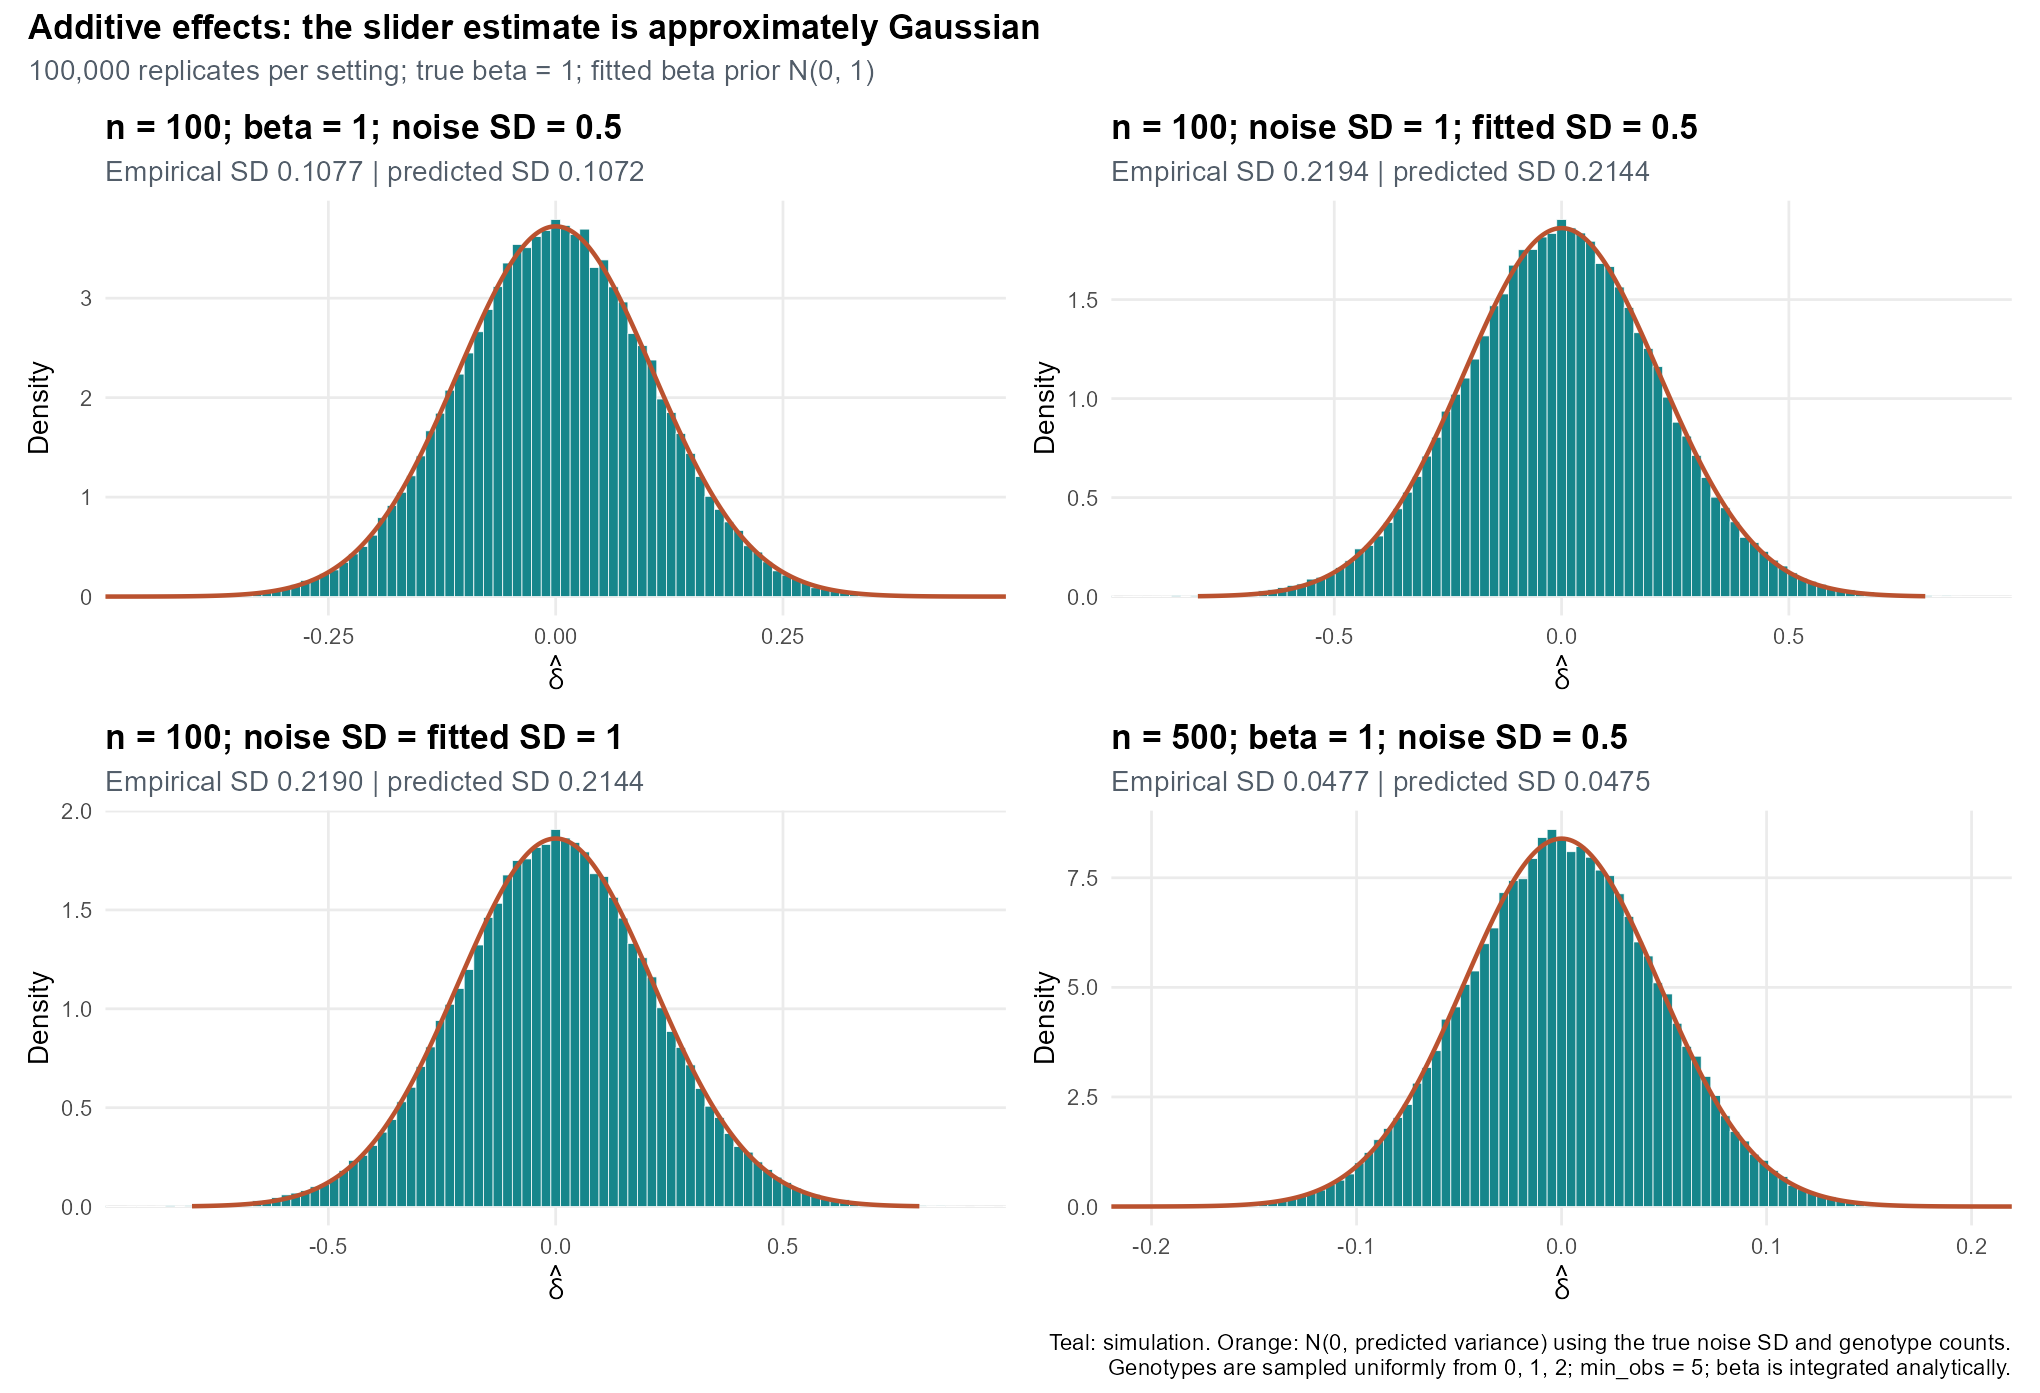
\includegraphics[width=\textwidth]{additive_delta_histograms.png}
\caption{Empirical distributions of the estimated slider under
additivity (histograms), with zero-centered Gaussian densities
whose variances are predicted from the true effect, true noise,
and genotype counts (curves). Each panel uses 100,000 replicates,
true $\beta_*=1$, and the fitted prior $\beta\sim\Normal(0,1)$.}
\label{fig:additive-null-histograms}
\end{figure}

The five settings in Table~\ref{tab:additive-null} assess the
strong, fixed additive-effect regime for which the result is
derived. The simulation script also retains eight supplementary
settings with weak effects, sparse genotype classes, or redrawn
true effects; those settings are outside the focus of the
Gaussian approximation presented here.

\paragraph{Simulation from exact sufficient statistics.}
To avoid generating individual outcomes for every replicate,
we sampled genotype counts and independent group sums. Conditional
on counts and a specified true effect, these sums obey
\begin{equation}
U_g=\sum_{i:x_i=g}y_i
 =n_g(\alpha_*+\beta_*g)+\sigma_*\sqrt{n_g}\,Z_g,
\qquad Z_g\overset{\mathrm{iid}}{\sim}\Normal(0,1).
\end{equation}
This is an exact Gaussian sampling identity, not an approximation
to the distribution of $\widehat\delta$. The counts and sums
determine every crossproduct used by the estimator, including
$R_x=U_1+2U_2-\bar x\sum_g U_g$ and
$R_h=U_1-\bar h\sum_g U_g$. The compiled solver in
\texttt{susieSlide} was used to maximize the same one-SNP
marginal objective, with no predictor standardization. Its results
were checked against \texttt{slider::linearized\_snp} on 400
full individual-level datasets spanning weak and strong effects,
rare classes, different prior and noise variances, and enabled
or disabled count filtering. The maximum absolute difference
in the estimated slider was approximately $1.34\times10^{-12}$.
The reproducible script is
\texttt{simulate\_slider\_additive\_null.R}.

\clearpage
\section{R interface and scope}

The one-SNP estimation and testing routines are defined in
\texttt{slider\_model.R}. They require only base R. The minimal
implementation accepts finite numeric phenotype values and hard-call
genotypes in $\{0,1,2\}$. Missing observations and continuous genotype dosages are
not accepted. The arguments \texttt{sigma} and \texttt{sigma0} are
standard deviations, not variances.

The parameter \texttt{min\_obs}, equal to 5 by default, controls a
sparse-category fallback. Let $n_k=\sum_i\ind_{\{x_i=k\}}$ for
$k\in\{0,1,2\}$. If $\min(n_0,n_1,n_2)<\texttt{min\_obs}$, the
implementation fixes $\delta=0$ and skips marginal-likelihood
optimization over $\delta$. A missing category has count zero and
therefore activates this rule. Exactly five observations in each
category passes the default threshold. The conditional posterior
for $\beta$ is still calculated under the same Gaussian prior,
using additive coding $(0,1,2)$. The rule overrides \texttt{gam};
setting \texttt{min\_obs=0} disables it. The threshold must be a
nonnegative integer. The fallback preserves any observed genotype
contrast and, with an intercept, gives the same fitted values and
evidence after switching the counted allele. It imposes additivity
when counts are sparse rather than establishing evidence for additivity.

\begin{lstlisting}
source("slider_model.R")

set.seed(1)
n_sim <- 1000
x <- sample(0:2, replace = TRUE, size = n_sim)
y <- rnorm(n_sim, sd = 0.5)
y[x == 1] <- y[x == 1] + 0.2
y[x == 2] <- y[x == 2] + 0.7

# Estimate delta; integrate beta under its Gaussian prior.
out <- linearized_snp(y, x, sigma = 0.5, sigma0 = 1, min_obs = 5)
out$delta
out$beta_mean
out$beta_sd

# Fit a specified coding: gam is the fixed value of delta.
additive <- linearized_snp(y, x, sigma = 0.5,
                          sigma0 = 1, gam = 0)

# Optional additivity comparison with equal prior model odds.
comparison <- slider_delta_test(out, prior_additive = 0.5)

# Fix the intercept at zero when this is the intended model.
zero_intercept <- linearized_snp(y, x, sigma = 0.5,
                                sigma0 = 1, intercept = FALSE)
\end{lstlisting}

When the count rule does not apply and \texttt{gam=NULL},
\texttt{delta} and \texttt{delta\_eb} both
contain the marginal-likelihood estimate. When \texttt{gam} is
specified and the count rule does not apply, \texttt{delta} is that
fixed value and all returned fitted quantities use it;
\texttt{delta\_eb} still records the unrestricted optimum on $[-1,1]$.
When the count rule applies, the returned \texttt{delta\_forced} is true,
\texttt{delta\_method} is \texttt{fixed (min\_obs)}, and
\texttt{delta\_eb} is \texttt{NA} because it was not estimated.
The output also includes \texttt{genotype\_counts} and
\texttt{min\_obs}. The testing routine reports an error for
count-forced fits rather than computing a nonadditivity comparison.
For other fits it compares the additive model with the integrated
uniform-slider model, independently of whether \texttt{gam} was
fixed in the preceding fit.

The output includes the conditional posterior mean, variance and
standard deviation of $\beta$, the intercept estimate, fitted values,
residuals, genotype means, and
\begin{equation}
\RSS=\sum_{i=1}^n\{y_i-\widehat y_i(\delta)\}^2.
\end{equation}
This reported $\RSS$ is evaluated at the posterior mean fit; it is
not the marginal-likelihood fitting objective or a posterior expected
residual sum of squares. The field
\texttt{log\_bf\_fixed\_delta} contains $\ell(\delta)$ at the
returned slider value. The function \texttt{at\_delta} evaluates
$m_\delta$, $V_\delta$, and $\ell(\delta)$ at supplied slider values.

At $\beta=0$, the sampling model contains no information about
$\delta$. Inheritance-mode estimates can therefore be poorly
determined for weak effects, even when the routine returns a unique
marginal-likelihood optimum. The one-SNP implementation reports a
point estimate of $\delta$ and a conditional posterior for $\beta$;
it does not report a credible interval for $\delta$ or a posterior
for $\beta$ averaged over slider uncertainty.

The base-R implementation described in this section fits a single
SNP and holds both $\sigma^2$ and $\sigma_0^2$ fixed. The multi-SNP
model, variable-selection probabilities, and component credible sets
are the separate VEB extension derived in
Section~\ref{sec:slider-veb}, implemented in \texttt{susieSlide}.
The separate numerical checks for the one-SNP routine verify the
fixed-slider formulas against direct Gaussian calculations, compare
the slider maximum with numerical searches across 100 simulated
cases, and check the integrated evidence, allele reversal, boundary
solutions, and strong-signal numerical stability.

\begin{thebibliography}{9}
\bibitem{wang2020susie}
Wang, G., Sarkar, A., Carbonetto, P., and Stephens, M. (2020).
A simple new approach to variable selection in regression, with
application to genetic fine mapping.
\emph{Journal of the Royal Statistical Society: Series B},
\textbf{82}(5), 1273--1300.
\href{https://doi.org/10.1111/rssb.12388}{doi:10.1111/rssb.12388}.

\bibitem{wang2018susie}
Wang, G., Sarkar, A., Carbonetto, P., and Stephens, M. (2018).
A simple new approach to variable selection in regression, with
application to genetic fine-mapping.
\emph{bioRxiv}, version 1, December 19, 2018.
Appendix B, especially Sections B.1--B.4 and Proposition 2.
\href{https://doi.org/10.1101/501114}{doi:10.1101/501114}.

\bibitem{oehlert1992delta}
Oehlert, G. W. (1992).
A note on the delta method.
\emph{The American Statistician}, \textbf{46}(1), 27--29.
\href{https://doi.org/10.1080/00031305.1992.10475842}
 {doi:10.1080/00031305.1992.10475842}.
\end{thebibliography}

\end{document}
